\section*{Additional Material}

\begin{frame}[noframenumbering]
    \centering
    \Huge{Additional Material}
\end{frame}

\begin{frame}[noframenumbering, label=ewsb]
\frametitle{Electroweak Symmetry Breaking}
\centering
\backto{sm2}{Standard Model}
\begin{columns}
\column{.5\textwidth}
Higgs mechanism:
\begin{itemize}
    \item Introduce potential $-\frac{1}{2} \mu^2|\phi|^2 +
        \frac{1}{4} \lambda^2 |\phi|^4$
    \item Expand around the vacuum expecation value, $v$, with
        fluctuations, $h$.
    \item Kinetic Lagrangian terms produce mass terms for the $W$ and
        $Z$ bosons.

\end{itemize}
\column{.5\textwidth}
\begin{figure}
\centering
\includegraphics[width=\textwidth]{higgspotential.png}
\end{figure}
\end{columns}
\end{frame}

\begin{frame}[noframenumbering, label=pdfs]
\frametitle{Parton Distribution Functions}
\begin{center}
    \backto{proton_collision}{proton collisions}
\end{center}
\begin{itemize}
    \item Protons are composite objects made up of quarks and gluons.
    \item Constituent partons interact directly in high energy
        collisions.
    \item Parton distribution functions (PDFs) describe the
        probability density $f(x)$ of a parton with relative momentum
        fraction, $x=p_{parton}/p_{proton}$.
\end{itemize}

\vfill

\begin{figure}
\centering
\includegraphics[height=4cm]{pdfs.png}
\end{figure}
\end{frame}

\begin{frame}[noframenumbering, label=topprops]
    \frametitle{Top Quark Properties}
\begin{itemize}
    \item $m_{top} = 173.5 \pm 0.6 \pm 0.8$~GeV
    \item $\Gamma \approx 1.29$~GeV
    \item $\tau \approx 0.5 \times 10^{-24}$~s
    \item $\ttbar \to$ hadrons: 45.7\%
    \item $\ttbar \to \ell +$jets: 43.8\%
    \item $\ttbar \to \ell\ell$: 10.5\%
\end{itemize}

\centering
\backto{whytopquarks}{why top quarks?}
\end{frame}

\subsubsection*{Models Beyond the Standard Model}

\subsubsection*{Extra Dimensions}
\label{extradims}

\begin{frame}[noframenumbering]
\frametitle{Extra Dimensions and the Hierarchy Problem}
\begin{columns}
\column{.5\textwidth}
\centering
\backto{strat2}{Analysis Strategy}
\begin{figure}
\includegraphics[width=\textwidth]{kaluzaklein.png}
\end{figure}
\column{.5\textwidth}
\begin{itemize}
    \item To address the hierarchy problem, some models add a new
        spatial dimension which gravity ``leaks'' into.
    \item Gauss's law for gravity in 3+1 dimensions makes Newton's
        constant appear small.
    \item Momentum in the extra dimension will manifest as apparent
        mass, and the spectrum will be discrete if the extra
        dimension is finite (Kaluza-Klein excitation).
\end{itemize}
\end{columns}
\end{frame}

\begin{frame}[noframenumbering, label=rskkg]
\frametitle{Randall-Sundrum Warped Extra Dimensions}
\begin{itemize}
    \item Randall-Sundrum Warped Extra Dimension models introduce a
        new spatial dimension with a curved metric:
\begin{equation*}
    ds^2 = e^{-2k|y|} \eta_{\mu\nu} dx^\mu dx^\nu - dy^2.
\end{equation*}

    \item The extra dimension is parameterized by $y$ and has
        curvature $k$, and it connects the usual space-time infrared
        brane (at $y = r$) to the Planck scale ultraviolet brane (at
        $y = 0$).

    \item Observed particle masses $m$ are related to the fundamental
        masses $m_0$ by $m = e^{kr\pi} m_0$.

    \item Standard Model particles are mostly localized near the UV
        brane to account for their low mass; the top quark is
        localized nearest to the IR brane.

    \item Excitations of the gluon field in the extra dimension are
        localized near the IR brane and therefore couple most strongly
        to top quarks.

\end{itemize}
\end{frame}


\subsubsection*{Topcolor Assisted Technicolor}
\label{topcolor}

\begin{frame}[noframenumbering]
\frametitle{Topcolor Assisted Technicolor}
\begin{center}
\backto{strat2}{Analysis Strategy}
\end{center}
\begin{itemize}
    \item The top quark's mass suggests a role in EWSB.
    \item Topcolor assisted technicolor models introduce additional
        symmetry groups which are broken to yield the SM: SU(3)$_1
        \times$U(1)$_1 \times$SU(3)$_2 \times $U(1)$_2
        \times$SU(2)$\to$SU(3)$\times$SU(2)$\times$U(1).
    \item The new SU(3)$_i \times$U(1)$_i$ couple preferentially to
        different generations of fermions.
    \item The inclusion of a new broken U(1) symmetry group gives rise
        to a new massive neutral vector boson, $Z^\prime$.
    \item Some freedom in the model: if one set of symmetries couples
        preferentially to generations 1 and 3, this yields the largest
        cross section times branching ratio to \ttbar\ pairs at the
        LHC.
\end{itemize}
\end{frame}

\begin{frame}[noframenumbering]
    \frametitle{Boosted Event Yields}
    \centering
\begin{tabular}{lr@{$~\pm~$}rr@{$~\pm~$}rr@{$~\pm~$}r}
\hline
\multicolumn{7}{c}{Boosted selection} \\
& \multicolumn{2}{c}{$e$}  & \multicolumn{2}{c}{$\mu$} & \multicolumn{2}{c}{Sum} \\
\hline
\hline
\ttbar\ & 2100 &  500 & 2800 &  600 & 4900 &  1100 \\ \hline
Single top & 71 &  15 & 105 &  22 & 176 &  34 \\ \hline
Multi-jet & 39 &  19 & 32 &  16 & 71  & 25  \\ \hline
$W$+jets & 170 &  60 & 310 &  90 & 480 &  140 \\ \hline
$Z$+jets & 18 &  11 & 33 &  8 & 52 &  15 \\ \hline
Di-bosons & 2.0 &  0.8 & 1.5 &  1.4 & 3.5 &  1.8 \\ \hline
Total & 2400 &  500 & 3300 &  700 & 5600 &  1200 \\ \hline
Data  & 2177 & 47 & 2945  & 54 & 5122 & 72 \\ \hline
\hline
\end{tabular}

Systematic uncertainties are included.
\end{frame}

\begin{frame}[noframenumbering]
    \frametitle{Resolved Event Yields}
    \centering
\begin{tabular}{lr@{$~\pm~$}rr@{$~\pm~$}rr@{$~\pm~$}r}
\hline
\multicolumn{7}{c}{Resolved selection} \\
& \multicolumn{2}{c}{$e$}  & \multicolumn{2}{c}{$\mu$} & \multicolumn{2}{c}{Sum} \\
\hline 
\hline
\ttbar\ & 94000 &  15000 & 118000 &  19000 & 211000 &  33000 \\ \hline
Single top & 6800 &  800 & 8400 &  1100 & 15200 &  1900 \\ \hline
Multi-jet & 3700 &  1800 & 10000 &  5000 & 14000 &  6000 \\ \hline
$W$+jets & 16000 &  4000 & 23000 &  6000 & 39000 &  10000 \\ \hline
$Z$+jets & 1800 &  400 & 1800 &  400 & 3600 &  800 \\ \hline
Di-bosons & 230 &  50 & 320 &  60 & 550 &  100 \\ \hline
Total & 121000 &  17000 & 162000 &  23000 & 283000 &  39000 \\ \hline
Data  & 119490 & 346 & 160878  & 401 & 280251 & 529 \\ \hline
\hline
\end{tabular}
Systematic uncertainties are included.
\end{frame}


\begin{frame}[t, noframenumbering, label=jet_clustering]
    \frametitle{Jet Clustering Algorithms}
    \centering
    \backto{jet_reco}{jet reconstruction}
    \begin{align*}
        d_{ij} = & \min(k_{ti}^{2p}, k_{tj}^{2p})
        \frac{\dr_{ij}^2}{R^2} \\
        d_{iB} = & k_{ti}^{2p}
    \end{align*}

    \begin{columns}

    \column{.5\textwidth}
    \begin{figure}
    \centering
    \includegraphics[width=.8\textwidth]{kt10.png}
    \end{figure}

    \column{.5\textwidth}
    \begin{figure}
    \centering
    \includegraphics[width=.8\textwidth]{akt10.png}
    \end{figure}

\end{columns}

\end{frame}

\begin{frame}[noframenumbering,label=trimming]
    \frametitle{Jet Trimming Procedure}
\begin{figure}
\centering
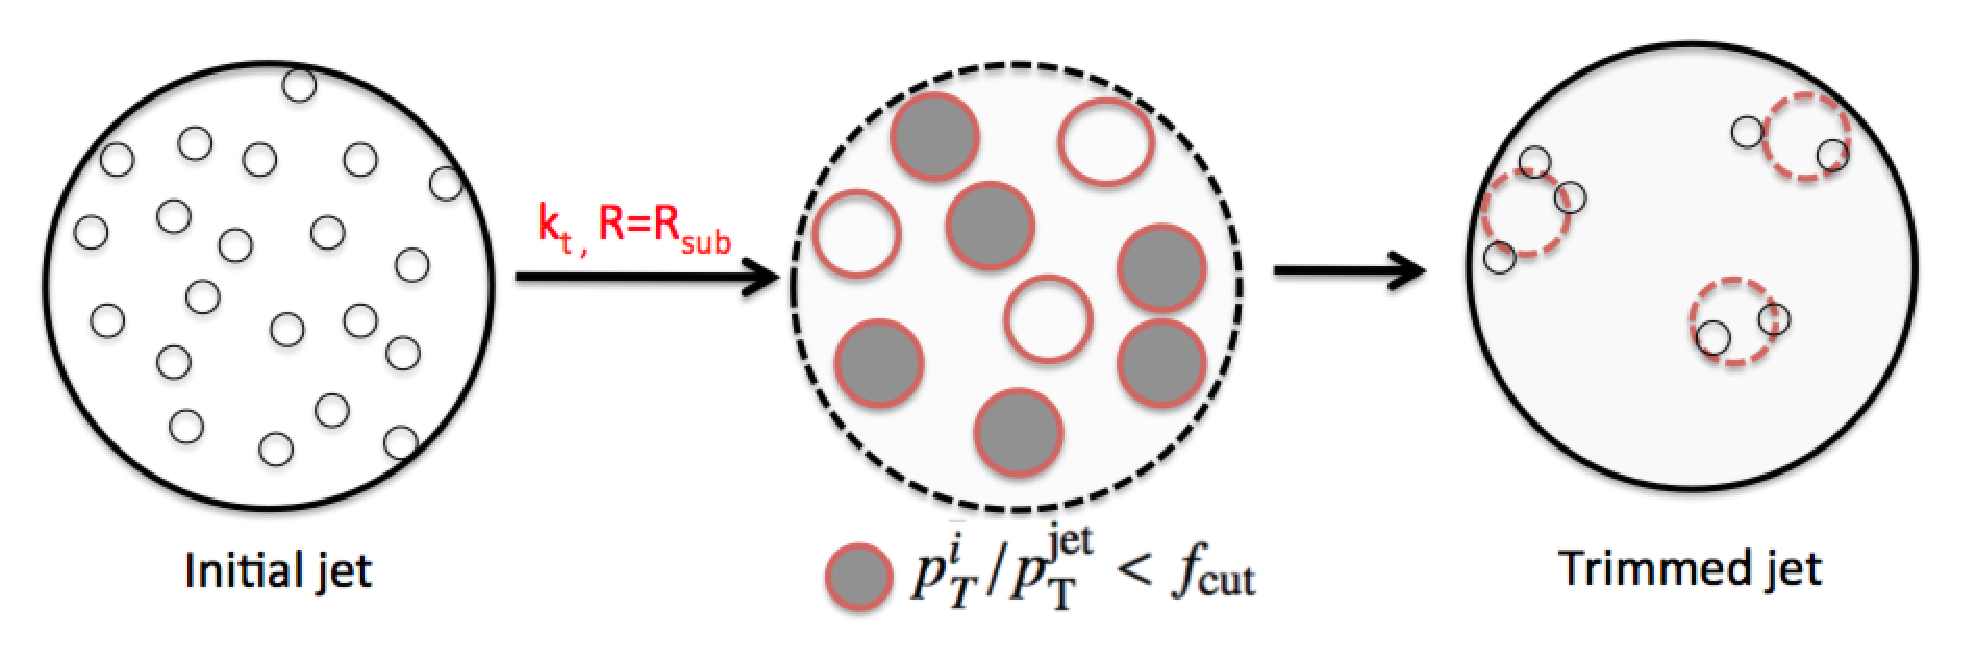
\includegraphics[width=.5\textwidth]{trimscheme.eps}
\end{figure}
\begin{columns}
\column{.5\textwidth}
\begin{figure}
\centering
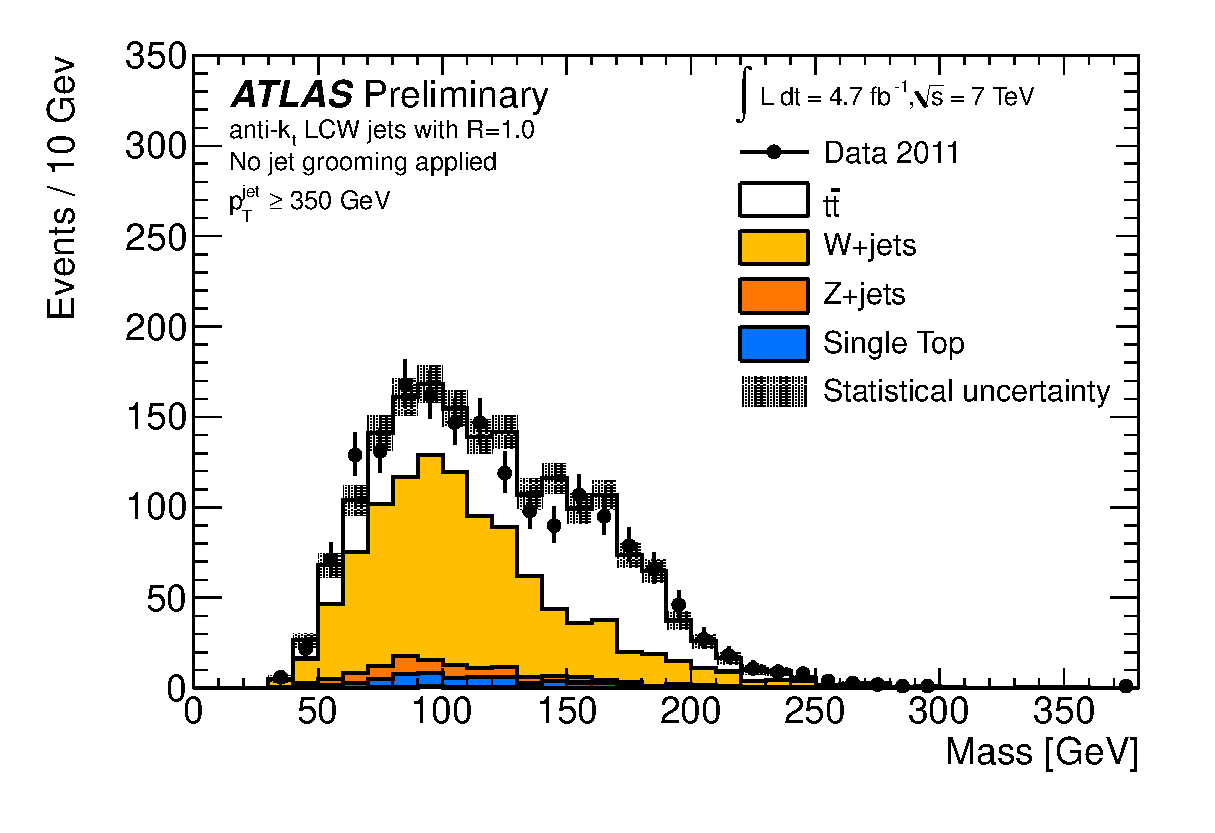
\includegraphics[width=\textwidth]{untrimmedtopjetmass.eps}
\end{figure}
\column{.5\textwidth}
\begin{figure}
\centering
\includegraphics[width=\textwidth]{trimmedtopjetmass.eps}
\end{figure}
\end{columns}
    \centering
    $f_{cut} = 0.05$; $R_{sub} = 0.3$
    \backto{boostedsel}{boosted selection}
\end{frame}


\begin{frame}[noframenumbering,label=btagging]
    \frametitle{$b$-tagging}
    \centering
    \backto{boostedsel}{boosted selection}
\begin{columns}
\column{.5\textwidth}
\begin{figure}
\centering
\includegraphics[width=\textwidth]{btageff.eps}
\end{figure}
\column{.5\textwidth}
\begin{figure}
\centering
\includegraphics[width=\textwidth]{btagsf.eps}
\end{figure}
\end{columns}
\end{frame}

\begin{frame}[noframenumbering,label=boostedjes]
    \frametitle{Jet Energy Scale Uncertainty}
    \centering
    \backto{systematics}{systematic uncertainties}
\begin{columns}
\column{.5\textwidth}
\begin{figure}
\centering
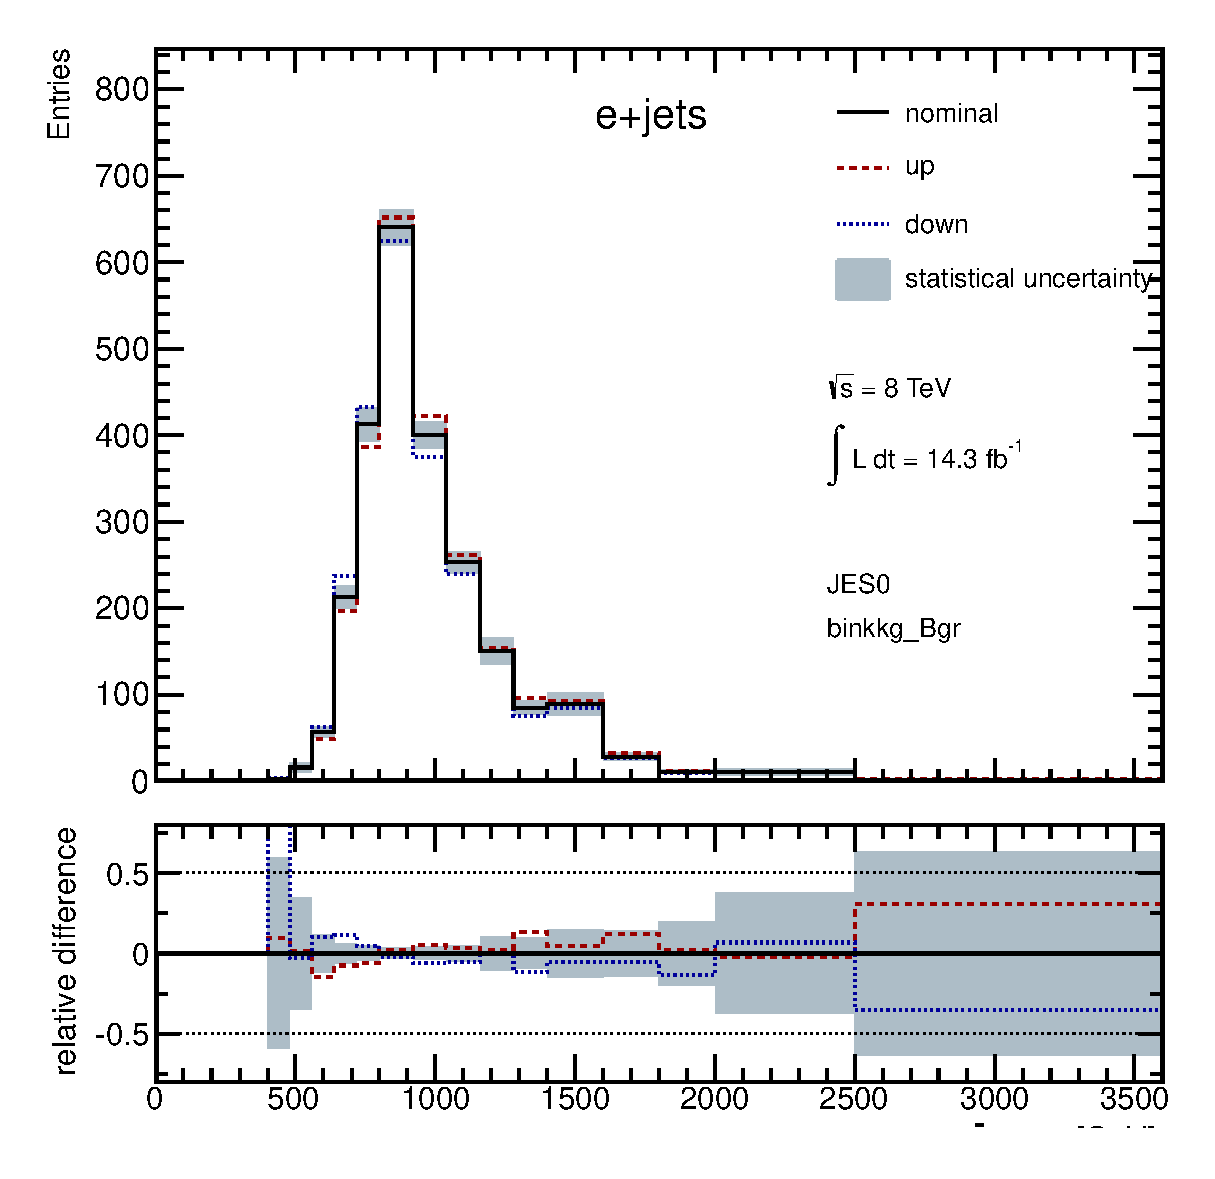
\includegraphics[width=\textwidth]{ejetsjes.eps}
\end{figure}
\column{.5\textwidth}
\begin{figure}
\centering
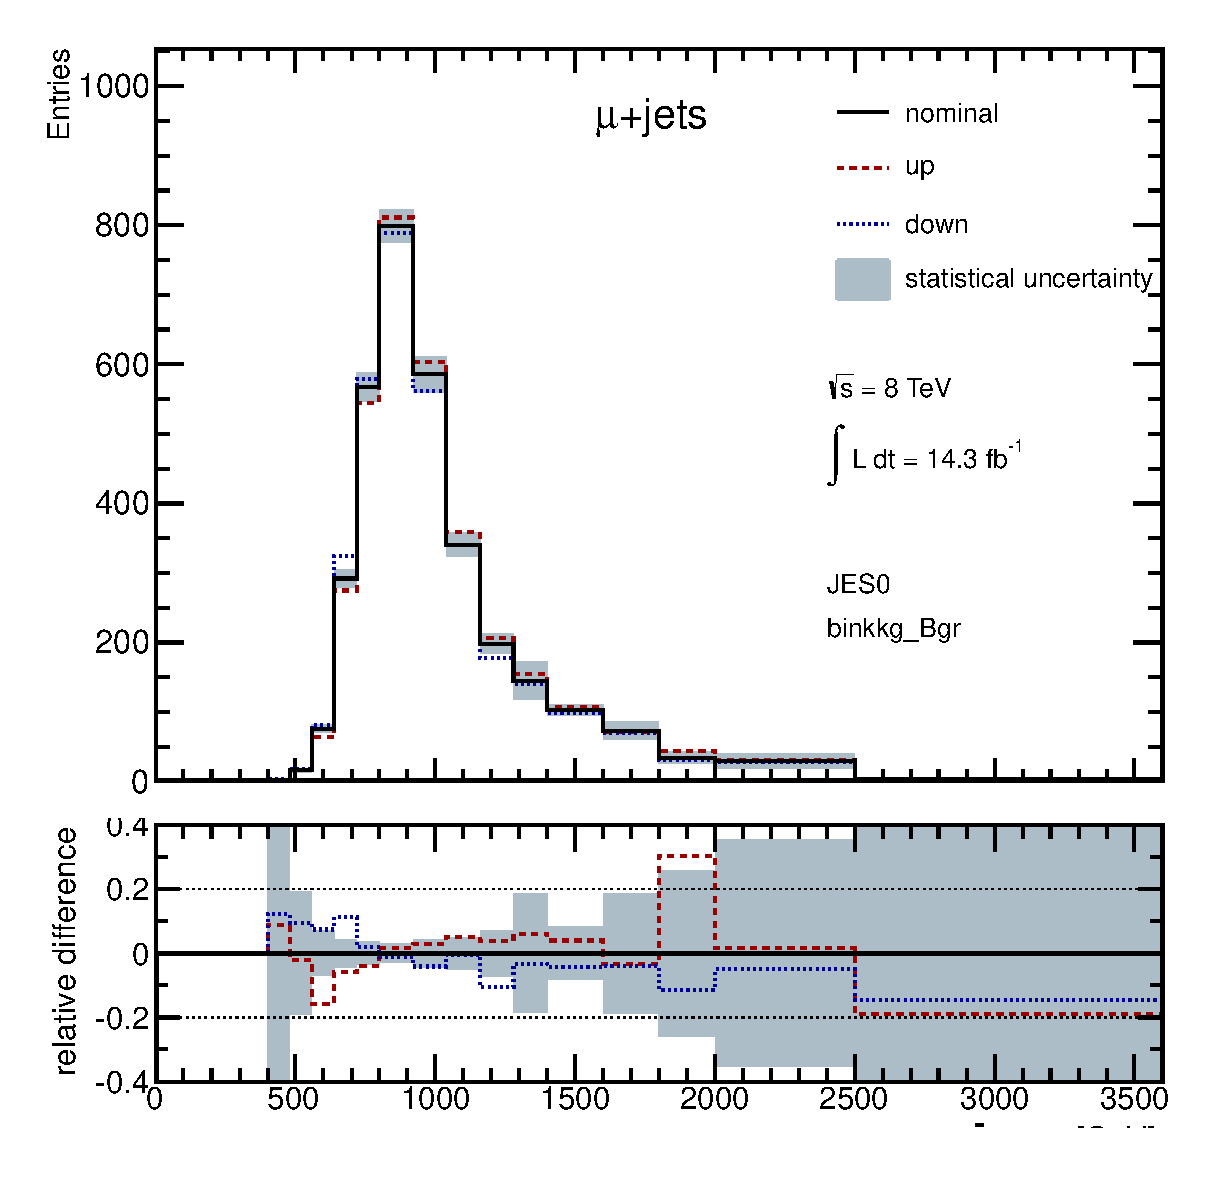
\includegraphics[width=\textwidth]{mujetsjes.eps}
\end{figure}
\end{columns}
\end{frame}

\begin{frame}[noframenumbering,label=bethebloch]
    \frametitle{Stopping Power}
\begin{figure}
\centering
\includegraphics[width=\textwidth]{bethebloch.png}
\end{figure}
\end{frame}

\begin{frame}[noframenumbering]
    \frametitle{Upgrade Software Framework}
\begin{figure}
\centering
\includegraphics[width=\textwidth]{upgradeframe.png}
\end{figure}
\end{frame}


\subsubsection*{BSM Vector Boson Scattering}

\begin{frame}[noframenumbering]
    \frametitle{BSM Vector Boson Scattering}
    \centering
\begin{figure}
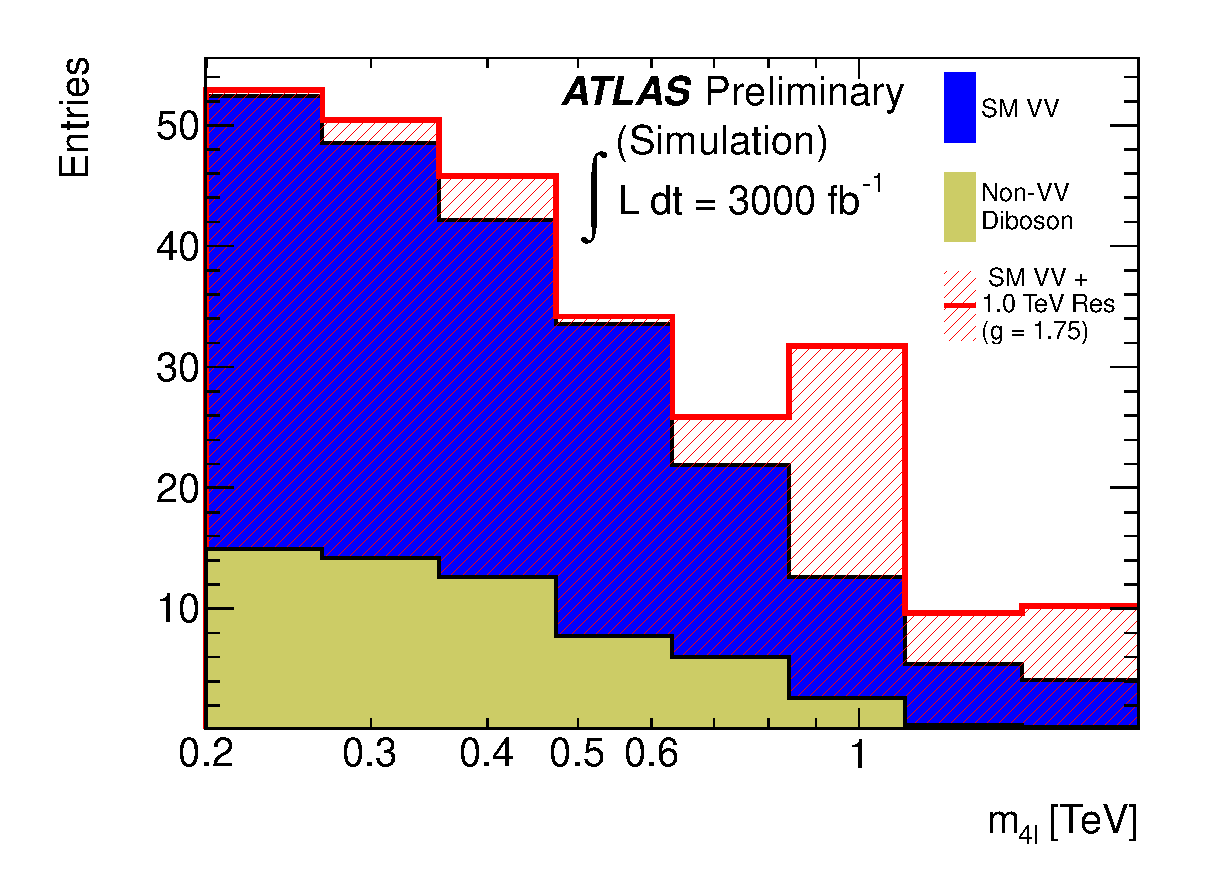
\includegraphics[width=0.5\textwidth]{log10_m_llll_f_m1000_g175_zz_v3.eps}
\end{figure}

\begin{tabular}{lcc} \hline  model              & $300\,\ifb$  & $3000\,\ifb$  \\ 
\hline $m_{\rm resonance} = 500$~GeV, $g = 1.0$ &  $ 2.4 \sigma$  & $7.5 \sigma$  \\ 
\hline $m_{\rm resonance} = 1$~TeV, $g = 1.75$ &  $ 1.7 \sigma$  & $5.5 \sigma$  \\ 
\hline $m_{\rm resonance} = 1$~TeV, $g = 2.5$ &  $ 3.0 \sigma$  & $9.4 \sigma$  \\ 
\hline \hline
\end{tabular}

\vspace{10pt}

Expected deviations from the SM
\end{frame}

\subsection*{BSM Higgs Resonances}

\begin{frame}[noframenumbering]
    \frametitle{BSM Higgs Resonances}
\centering
\begin{figure}
    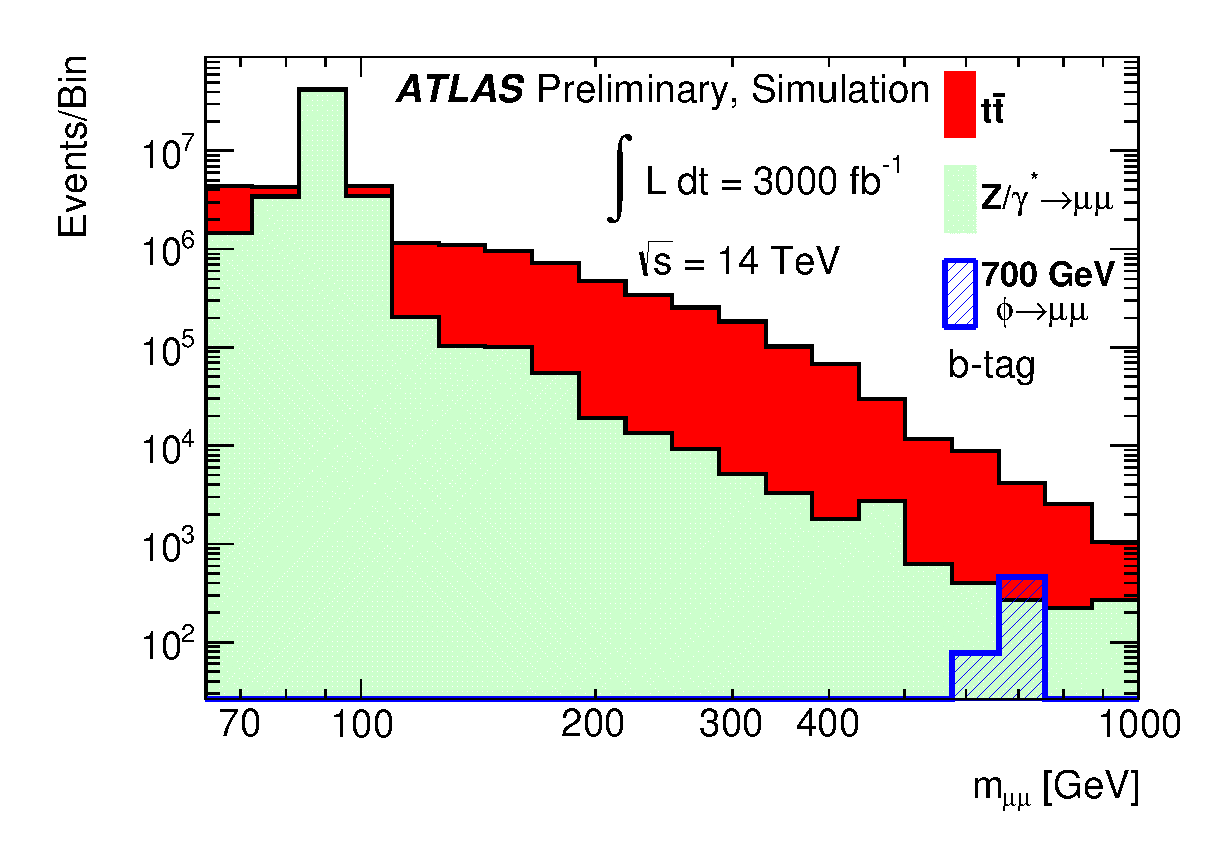
\includegraphics[height=5cm]{bbAmumu700.eps}
    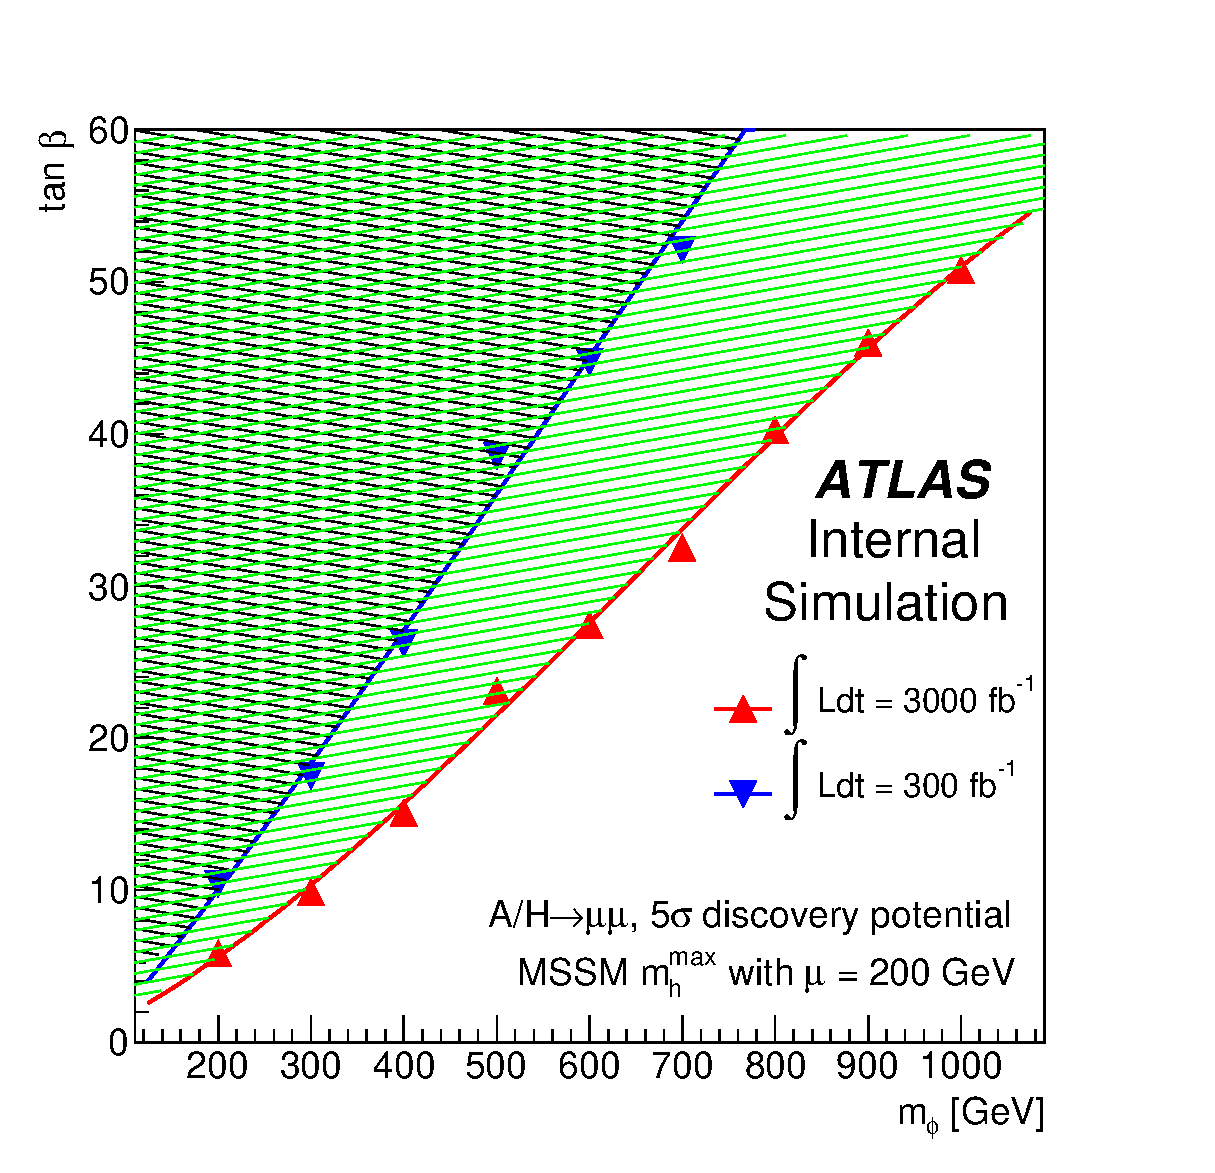
\includegraphics[height=5cm]{tanBeta_Vs_mA_combined.eps}
\end{figure}

\vspace{15pt}
\noindent $m_{\mu\mu}$ spectra and expected $5\sigma$ discovery contours
for the $H/A \to \mu\mu$ search
\end{frame}
